\begin{frame}
	\myheading{Module 7.1:  Introduction to Autoencoders }
\end{frame}


\begin{frame}
	\begin{columns}  
    		\column{0.5\textwidth}    
    		\begin{overlayarea}{\textwidth}{\textheight}        
        		\vspace{5pt}
			\tikzstyle{input_neuron}=[circle,draw=red!50,fill=red!10,thick,minimum size=6mm]
\tikzstyle{hidden_neuron}=[circle,draw=blue!50,fill=cyan!10,thick,minimum size=6mm]
\tikzstyle{output_neuron}=[circle,draw=green!50,fill=green!10,thick,minimum size=6mm]
\tikzstyle{input}=[circle,draw=black!50,fill=black!20,thick,minimum size=6mm]

\begin{center}
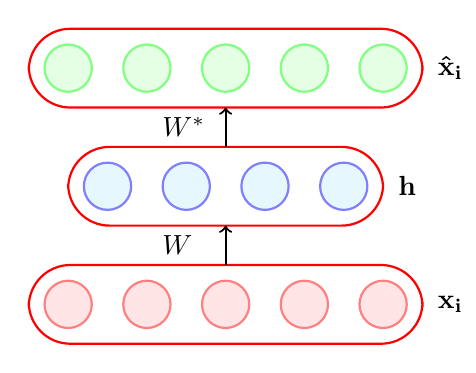
\begin{tikzpicture}

\node [input_neuron] (neuron01) at (6.5,4.5) {};
\node [input_neuron] (neuron02) at (7.5,4.5){};
\node [input_neuron] (neuron03) at (8.5,4.5) {};
\node [input_neuron] (neuron04) at (9.5,4.5) {};
\node [input_neuron] (neuron05) at (10.5,4.5) {};
\node [hidden_neuron] (neuron51) at (7,6) {} ;
\node [hidden_neuron] (neuron52) at (8,6)  {};
\node [hidden_neuron] (neuron53) at (9,6)  {};
\node [hidden_neuron] (neuron54) at (10,6)  {};

\node [output_neuron] (neuron11) at (6.5,7.5)  {};
\node [output_neuron] (neuron12) at (7.5,7.5)  {};
\node [output_neuron] (neuron13) at (8.5,7.5)  {};
\node [output_neuron] (neuron14) at (9.5,7.5)  {};
\node [output_neuron] (neuron15) at (10.5,7.5)  {};

\node[text width=0.01cm] at (11.2,4.5) {$\mathbf{x_i}$};
\node[text width=0.007cm] at (7.7,5.25) {$W$};
\node[text width=0.01cm] at (10.7,6) {$\mathbf{h}$};
\node[text width=0.007cm] at (7.7,6.75) {$W^*$};
\node[text width=0.01cm] at (11.2,7.5) {$\mathbf{\hat{x}_i}$};

\draw[red!100,thick,solid,rounded corners=15pt] (6,4) rectangle (11,5);
\draw[red!100,thick,solid,rounded corners=15pt] (6.5,5.5) rectangle (10.5,6.5);
\draw[red!100,thick,solid,rounded corners=15pt] (6,7) rectangle (11,8);

\draw[thick,->] (8.5,5) -- (8.5,5.5);

\draw[thick,->] (8.5,6.5) -- (8.5,7);


\end{tikzpicture}
\end{center}
                
        		\vspace{-24pt}

			\begin{align*}
				\onslide<4->{\mathbf{h} &= g(W\mathbf{x_i} + \mathbf{b})}\\
				\onslide<6->{\mathbf{\hat{x}_i} &= f(W^*\mathbf{h} + \mathbf{c} )}
			\end{align*}

			\if 0
				\only<4->
					{
	            			\begin{align*}
    		        				\mathbf{h} = g(W\mathbf{x_i} +\mathbf{b})
	        		    	\end{align*}
    	    		}
    		    	\vspace{-0.5cm}
        			\only<6->
        			{
	            		\begin{align*}
						    \hspace{1.25cm}
	        			    \mathbf{\hat{x}_i} = f(W^*\mathbf{h} +\mathbf{c})
            			\end{align*}            
	        		}
			\fi 

    		\end{overlayarea}
    
    		\column{0.5\textwidth}
    
    		\begin{overlayarea}{\textwidth}{\textheight}
	       \only<2->
	       {
    		   \begin{itemize}\justifying
    					%\item<1-> We will assume a Dataset with $m$ examples and each example has $n$ dimensions.
		%			\item<1-> $x_{ij}$ : $j^{th}$ dimension of $i^{th}$ example.
	               \item<2-> An autoencoder is a special type of feed forward neural network which does the following
                    \item<3-> \underline{Encodes} its input $\mathbf{x_i}$ into a hidden representation $\mathbf{h}$
                    \item<5-> \underline{Decodes} the input again from this hidden representation
            		\item<7-> The model is trained to minimize a certain loss function which will ensure that $\mathbf{\hat{x}_i}$ is close to $\mathbf{x_i}$ (we will see some such loss functions soon)
        		\end{itemize}
            }
    
    		\end{overlayarea}    
  	\end{columns}
\end{frame}


\begin{frame}
	\begin{columns}
    		\column{0.5\textwidth}
            \begin{overlayarea}{\textwidth}{\textheight}  
    		    \vspace{5.27pt}
			    \tikzstyle{input_neuron}=[circle,draw=red!50,fill=red!10,thick,minimum size=6mm]
\tikzstyle{hidden_neuron}=[circle,draw=blue!50,fill=cyan!10,thick,minimum size=6mm]
\tikzstyle{output_neuron}=[circle,draw=green!50,fill=green!10,thick,minimum size=6mm]
\tikzstyle{input}=[circle,draw=black!50,fill=black!20,thick,minimum size=6mm]

\begin{center}
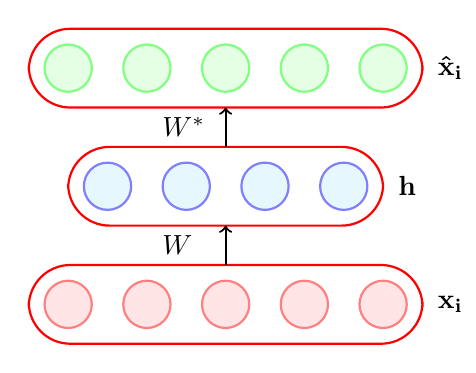
\begin{tikzpicture}

\node [input_neuron] (neuron01) at (6.5,4.5) {};
\node [input_neuron] (neuron02) at (7.5,4.5){};
\node [input_neuron] (neuron03) at (8.5,4.5) {};
\node [input_neuron] (neuron04) at (9.5,4.5) {};
\node [input_neuron] (neuron05) at (10.5,4.5) {};
\node [hidden_neuron] (neuron51) at (7,6) {} ;
\node [hidden_neuron] (neuron52) at (8,6)  {};
\node [hidden_neuron] (neuron53) at (9,6)  {};
\node [hidden_neuron] (neuron54) at (10,6)  {};

\node [output_neuron] (neuron11) at (6.5,7.5)  {};
\node [output_neuron] (neuron12) at (7.5,7.5)  {};
\node [output_neuron] (neuron13) at (8.5,7.5)  {};
\node [output_neuron] (neuron14) at (9.5,7.5)  {};
\node [output_neuron] (neuron15) at (10.5,7.5)  {};

\node[text width=0.01cm] at (11.2,4.5) {$\mathbf{x_i}$};
\node[text width=0.007cm] at (7.7,5.25) {$W$};
\node[text width=0.01cm] at (10.7,6) {$\mathbf{h}$};
\node[text width=0.007cm] at (7.7,6.75) {$W^*$};
\node[text width=0.01cm] at (11.2,7.5) {$\mathbf{\hat{x}_i}$};

\draw[red!100,thick,solid,rounded corners=15pt] (6,4) rectangle (11,5);
\draw[red!100,thick,solid,rounded corners=15pt] (6.5,5.5) rectangle (10.5,6.5);
\draw[red!100,thick,solid,rounded corners=15pt] (6,7) rectangle (11,8);

\draw[thick,->] (8.5,5) -- (8.5,5.5);

\draw[thick,->] (8.5,6.5) -- (8.5,7);


\end{tikzpicture}
\end{center}
        
                \vspace{-10.5pt}
    		    \begin{align*}
        		        \mathbf{h} &= g(W\mathbf{x_i} +\mathbf{b})\\
            		   \mathbf{\hat{x}_i} &= f(W^*\mathbf{h} +\mathbf{c})
        		\end{align*}                

        
        		\begin{block}<6->{}
            		\justifying
            		\fontsize{10pt}{7.2}\selectfont
            		An autoencoder where $\text{dim}(\mathbf{h})<\text{dim}(\mathbf{x_i})$ is called an \underline{under complete} autoencoder
        		\end{block}
    		\end{overlayarea}

    		\column{0.5\textwidth}
    		\begin{overlayarea}{\textwidth}{\textheight}
    			\only<2->
    			{
	        		\begin{itemize}\justifying
        		    	\item<2-> Let us consider the case where $\text{dim}(\mathbf{h})<\text{dim}(\mathbf{x_i})$
            			\item<3-> If we are still able to reconstruct $\mathbf{\hat{x}_i}$ perfectly from $\mathbf{h}$, then what does it say about $\mathbf{h}$?
            			\item<4-> $\mathbf{h}$ is a loss-free encoding of $\mathbf{x_i}$. It captures all the important characteristics of $\mathbf{x_i}$
            			\item<5-> Do you see an analogy with PCA?
        			\end{itemize}
    			}
    		\end{overlayarea}  
  	\end{columns}
\end{frame}


\begin{frame}
	\begin{columns}
    	\column{0.5\textwidth}
   		\begin{overlayarea}{\textwidth}{\textheight}
    			\only<1->
    			{
	        		\vspace{3pt}
		      		\tikzstyle{input_neuron}=[circle,draw=red!50,fill=red!10,thick,minimum size=6mm]
\tikzstyle{hidden_neuron}=[circle,draw=blue!50,fill=cyan!10,thick,minimum size=6mm]
\tikzstyle{output_neuron}=[circle,draw=green!50,fill=green!10,thick,minimum size=6mm]
\tikzstyle{cpy_neuron}=[circle,draw=red!50,fill=red!50,thick,minimum size=6mm]
\tikzstyle{input}=[circle,draw=black!50,fill=black!20,thick,minimum size=6mm]

\begin{center}
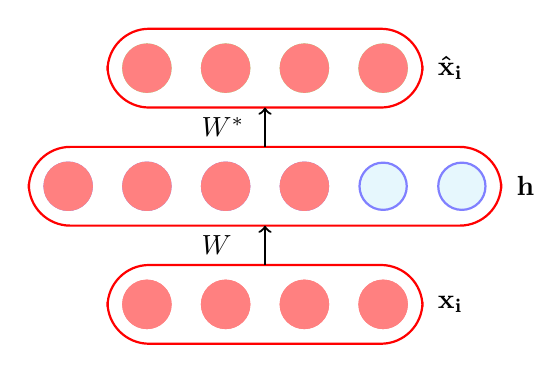
\begin{tikzpicture}

\node [input_neuron] (neuron01) at (8.5,4.5) {};
\node [input_neuron] (neuron02) at (9.5,4.5){};
\node [input_neuron] (neuron03) at (10.5,4.5) {};
\node [input_neuron] (neuron04) at (11.5,4.5) {};
\node [hidden_neuron] (neuron51) at (7.5,6) {} ;
\node [hidden_neuron] (neuron52) at (8.5,6)  {};
\node [hidden_neuron] (neuron53) at (9.5,6)  {};
\node [hidden_neuron] (neuron54) at (10.5,6)  {};
\node [hidden_neuron] (neuron55) at (11.5,6)  {};
\node [hidden_neuron] (neuron56) at (12.5,6)  {};

\node [output_neuron] (neuron11) at (8.5,7.5)  {};
\node [output_neuron] (neuron12) at (9.5,7.5)  {};
\node [output_neuron] (neuron13) at (10.5,7.5)  {};
\node [output_neuron] (neuron14) at (11.5,7.5)  {};


\node[text width=0.01cm] at (12.2,4.5) {$\mathbf{x_i}$};
\node[text width=0.007cm] at (9.2,5.25) {$W$};
\node[text width=0.01cm] at (13.2,6) {$\mathbf{h}$};
\node[text width=0.007cm] at (9.2,6.75) {$W^*$};
\node[text width=0.01cm] at (12.2,7.5) {$\mathbf{\hat{x}_i}$};

\draw[red!100,thick,solid,rounded corners=15pt] (8,4) rectangle (12,5);
\draw[red!100,thick,solid,rounded corners=15pt] (7,5.5) rectangle (13,6.5);
\draw[red!100,thick,solid,rounded corners=15pt] (8,7) rectangle (12,8);


\draw[thick,->] (10,5) -- (10,5.5);

\draw[thick,->] (10,6.5) -- (10,7);

\onslide<4->{ \node [cpy_neuron] (neuron01) at (8.5,4.5) {};}
\onslide<4->{ \node [cpy_neuron] (neuron02) at (9.5,4.5){};}
\onslide<4->{ \node [cpy_neuron] (neuron03) at (10.5,4.5) {};}
\onslide<4->{ \node [cpy_neuron] (neuron04) at (11.5,4.5) {};}
\onslide<5->{ \node [cpy_neuron] (neuron61) at (7.5,6) {} ;}
\onslide<6->{ \node [cpy_neuron] (neuron62) at (8.5,6)  {};}
\onslide<7->{ \node [cpy_neuron] (neuron63) at (9.5,6)  {};}
\onslide<8->{ \node [cpy_neuron] (neuron64) at (10.5,6)  {};}

\onslide<9->{ \node [cpy_neuron] (neuron71) at (8.5,7.5)  {};}
\onslide<10->{ \node [cpy_neuron] (neuron72) at (9.5,7.5)  {};}
\onslide<11->{ \node [cpy_neuron] (neuron73) at (10.5,7.5)  {};}
\onslide<12->{ \node [cpy_neuron] (neuron74) at (11.5,7.5)  {};}

\end{tikzpicture}
\end{center}        
        			\vspace{-20pt}
            		\begin{align*}
            			\mathbf{h} &= g(W\mathbf{x_i} +\mathbf{b})\\
            		    \mathbf{\hat{x}_i} &=f(W^*\mathbf{h} +\mathbf{c})
            		\end{align*}
    			}

	    		\vspace{0.2cm}
    		    \begin{block}<14->{}
        		    \justifying
            		\fontsize{10pt}{7.2}\selectfont
            		An autoencoder where $\text{dim}(\mathbf{h})\geq \text{dim}(\mathbf{x_i})$ is called an \underline{over complete} autoencoder
                \end{block}
    	\end{overlayarea}

    	\column{0.5\textwidth}
    	\begin{overlayarea}{\textwidth}{\textheight}
        	\begin{itemize}\justifying
           		\item <2-> Let us consider the case when $\text{dim}(\mathbf{h})\geq \text{dim}(\mathbf{x_i})$
           		\item <3-> In such a case the autoencoder could learn a trivial encoding by simply copying $\mathbf{x_i}$ into $\mathbf{h}$ and then copying $\mathbf{h}$ into $\mathbf{\hat{x}_i}$
           		\item <13-> Such an identity encoding is useless in practice as it does not really tell us anything about the important characteristics of the data
        	\end{itemize}
    	\end{overlayarea}
  	\end{columns}
\end{frame}

\begin{frame}
    \begin{block}{The Road Ahead}
        \begin{itemize}\justifying
            \item <2-> Choice of $f(\mathbf{x_i})$ and $g(\mathbf{x_i})$
            \item <3-> Choice of loss function
        \end{itemize}
    \end{block}
\end{frame}


\begin{frame}
    \begin{block}{The Road Ahead}
        \begin{itemize}\justifying
            \item \textcolor{red}{Choice of $f(\mathbf{x_i})$ and $g(\mathbf{x_i})$}
            \item Choice of loss function
        \end{itemize}
    \end{block}
\end{frame}

\begin{frame}
    \begin{columns}
        \column{0.5\textwidth}
        \begin{overlayarea}{\textwidth}{\textheight}
            \tikzstyle{input_neuron}=[circle,draw=red!50,fill=red!10,thick,minimum size=6mm]
\tikzstyle{hidden_neuron}=[circle,draw=blue!50,fill=cyan!10,thick,minimum size=6mm]
\tikzstyle{output_neuron}=[circle,draw=green!50,fill=green!10,thick,minimum size=6mm]

\tikzstyle{input}=[circle,draw=black!50,fill=black!20,thick,minimum size=6mm]

\begin{center}
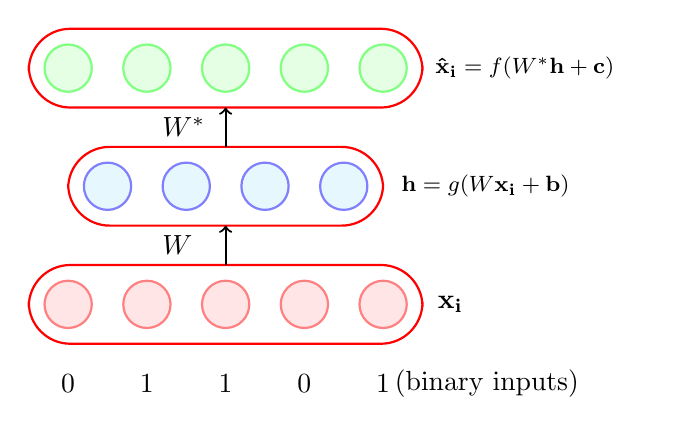
\begin{tikzpicture}

\node (input0) at (6.5,3.5) {0};
\node (input1) at (7.5,3.5) {1};
\node (input2) at (8.5,3.5){1};
\node (input3) at (9.5,3.5){0};
\node (input4) at (10.5,3.5){1};
\node [input_neuron] (neuron01) at (6.5,4.5) {};
\node [input_neuron] (neuron02) at (7.5,4.5){};
\node [input_neuron] (neuron03) at (8.5,4.5) {};
\node [input_neuron] (neuron04) at (9.5,4.5) {};
\node [input_neuron] (neuron05) at (10.5,4.5) {};
\node [hidden_neuron] (neuron51) at (7,6) {} ;
\node [hidden_neuron] (neuron52) at (8,6)  {};
\node [hidden_neuron] (neuron53) at (9,6)  {};
\node [hidden_neuron] (neuron54) at (10,6)  {};

\node [output_neuron] (neuron11) at (6.5,7.5)  {};
\node [output_neuron] (neuron12) at (7.5,7.5)  {};
\node [output_neuron] (neuron13) at (8.5,7.5)  {};
\node [output_neuron] (neuron14) at (9.5,7.5)  {};
\node [output_neuron] (neuron15) at (10.5,7.5)  {};

\node[text width=0.01cm] at (11.2,4.5) {$\mathbf{x_i}$};
\node[] at (11.8,6) {\footnotesize{$\mathbf{h}=g(W\mathbf{x_i}+\mathbf{b})$}};
\node[text width=0.007cm] at (7.7,5.25) {$W$};
%\node[] at (11.2,8.5) {$\hat{x} = f(W \times h(x) + c)$};
\node[text width=0.007cm] at (7.7,6.75) {$W^*$};
\node[] at (12.3,7.5) {\footnotesize{$\mathbf{\hat{x}_i}=f(W^*\mathbf{h}+\mathbf{c})$}};
\node[text width=3.1cm] at (12.2,3.5) {(binary inputs)};

\draw[red!100,thick,solid,rounded corners=15pt] (6,4) rectangle (11,5);
\draw[red!100,thick,solid,rounded corners=15pt] (6.5,5.5) rectangle (10.5,6.5);
\draw[red!100,thick,solid,rounded corners=15pt] (6,7) rectangle (11,8);

\draw[thick,->] (8.5,5) -- (8.5,5.5);

\draw[thick,->] (8.5,6.5) -- (8.5,7);


\end{tikzpicture}
\end{center}


            \begin{block}<8->{}
                $g$ is typically chosen as the sigmoid function
            \end{block}
        \end{overlayarea}

        \column{0.5\textwidth}
        \begin{overlayarea}{\textwidth}{\textheight}
            \begin{itemize}\justifying
                \item <2-> Suppose all our inputs are binary (each $x_{ij} \in \{0,1\}$)
                \item <3-> Which of the following functions would be most apt for the decoder?
                \begin{align*}
                    \onslide<4->{\mathbf{\hat{x}_i} &= \tanh (W^*\mathbf{h} +\mathbf{c} )} \\
                    \onslide<5->{\mathbf{\hat{x}_i} &= W^*\mathbf{h} +\mathbf{c}}\\
                    \onslide<6->{\mathbf{\hat{x}_i} &= logistic(W^*\mathbf{h} +\mathbf{c})}\\
                \end{align*}
                \vspace{-0.5in}
                \item <7-> Logistic as it naturally restricts all outputs to be between 0 and 1
            \end{itemize}
        \end{overlayarea}
    \end{columns}
\end{frame}

\begin{frame}
    \begin{columns}
        \column{0.5\textwidth}
        \begin{overlayarea}{\textwidth}{\textheight}
            \tikzstyle{input_neuron}=[circle,draw=red!50,fill=red!10,thick,minimum size=6mm]
\tikzstyle{hidden_neuron}=[circle,draw=blue!50,fill=cyan!10,thick,minimum size=6mm]
\tikzstyle{output_neuron}=[circle,draw=green!50,fill=green!10,thick,minimum size=6mm]

\tikzstyle{input}=[circle,draw=black!50,fill=black!20,thick,minimum size=6mm]

\begin{center}
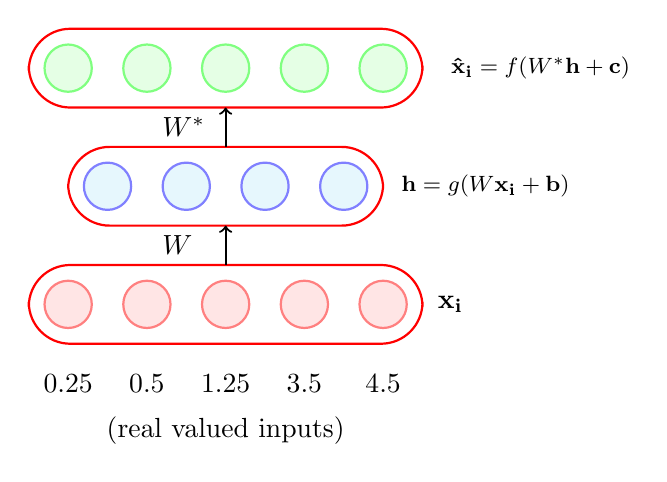
\begin{tikzpicture}

\node (input0) at (6.5,3.5) {0.25};
\node (input1) at (7.5,3.5) {0.5};
\node (input2) at (8.5,3.5){1.25};
\node (input3) at (9.5,3.5){3.5};
\node (input4) at (10.5,3.5){4.5};
\node [input_neuron] (neuron01) at (6.5,4.5) {};
\node [input_neuron] (neuron02) at (7.5,4.5){};
\node [input_neuron] (neuron03) at (8.5,4.5) {};
\node [input_neuron] (neuron04) at (9.5,4.5) {};
\node [input_neuron] (neuron05) at (10.5,4.5) {};
\node [hidden_neuron] (neuron51) at (7,6) {} ;
\node [hidden_neuron] (neuron52) at (8,6)  {};
\node [hidden_neuron] (neuron53) at (9,6)  {};
\node [hidden_neuron] (neuron54) at (10,6)  {};

\node [output_neuron] (neuron11) at (6.5,7.5)  {};
\node [output_neuron] (neuron12) at (7.5,7.5)  {};
\node [output_neuron] (neuron13) at (8.5,7.5)  {};
\node [output_neuron] (neuron14) at (9.5,7.5)  {};
\node [output_neuron] (neuron15) at (10.5,7.5)  {};

\node[text width=0.01cm] at (11.2,4.5) {$\mathbf{x_i}$};
\node[] at (11.8,6) {\footnotesize{$\mathbf{h}=g(W\mathbf{x_i}+\mathbf{b})$}};
\node[text width=0.007cm] at (7.7,5.25) {$W$};
%\node[] at (11.2,8.5) {$\hat{x} = f(W \times h(x) + c)$};
\node[text width=0.007cm] at (7.7,6.75) {$W^*$};
\node[] at (12.5,7.5) {\footnotesize{$\mathbf{\hat{x}_i}=f(W^*\mathbf{h}+\mathbf{c})$}};
\node[] at (8.5,2.9) {(real valued inputs)};

\draw[red!100,thick,solid,rounded corners=15pt] (6,4) rectangle (11,5);
\draw[red!100,thick,solid,rounded corners=15pt] (6.5,5.5) rectangle (10.5,6.5);
\draw[red!100,thick,solid,rounded corners=15pt] (6,7) rectangle (11,8);


\draw[thick,->] (8.5,5) -- (8.5,5.5);

\draw[thick,->] (8.5,6.5) -- (8.5,7);


\end{tikzpicture}
\end{center}

            \vspace{-20pt}
            \onslide<9->
            {
                \begin{block}{}
                    Again, $g$ is typically chosen as the sigmoid function
                \end{block}
            }
        \end{overlayarea}

        \column{0.5\textwidth}
        \begin{overlayarea}{\textwidth}{\textheight}
            \begin{itemize}\justifying
                \item <2-> Suppose all our inputs are real (each $x_{ij} \in \mathbb{R}$)
                \item <3-> Which of the following functions would be most apt for the decoder?
                \begin{align*}
                    \onslide<4->{\mathbf{\hat{x}_i} &= \tanh (W^*\mathbf{h} +\mathbf{c} )}\\
                    \onslide<5->{\mathbf{\hat{x}_i} &= W^*\mathbf{h} +\mathbf{c} } \\
                    \onslide<6->{\mathbf{\hat{x}_i} &= \text{logistic}(W^*\mathbf{h} +\mathbf{c})} \\
                \end{align*}
                \vspace{-0.5in}
                \item<7-> What will logistic and $\tanh$ do?
                \item<8-> They will restrict the reconstructed $\mathbf{\hat{x}_i}$ to lie between [0,1] or [-1,1] whereas we want $\mathbf{\hat{x}_i} \in \mathbb{R}^n$
            \end{itemize}
        \end{overlayarea}
    \end{columns}
\end{frame}

\begin{frame}
    \begin{block}{The Road Ahead}
        \begin{itemize}\justifying
            \item Choice of $f(\mathbf{x_i})$ and $g(\mathbf{x_i})$
            \item \textcolor{red}{Choice of loss function}
        \end{itemize}
    \end{block}
\end{frame}

\begin{frame}
	\footnotesize{
    \begin{columns}
        \column{0.5\textwidth}
        \begin{overlayarea}{\textwidth}{\textheight}
            \vspace{3pt}
            \tikzstyle{input_neuron}=[circle,draw=red!50,fill=red!10,thick,minimum size=6mm]
\tikzstyle{hidden_neuron}=[circle,draw=blue!50,fill=cyan!10,thick,minimum size=6mm]
\tikzstyle{output_neuron}=[circle,draw=green!50,fill=green!10,thick,minimum size=6mm]

\tikzstyle{input}=[circle,draw=black!50,fill=black!20,thick,minimum size=6mm]

\begin{center}
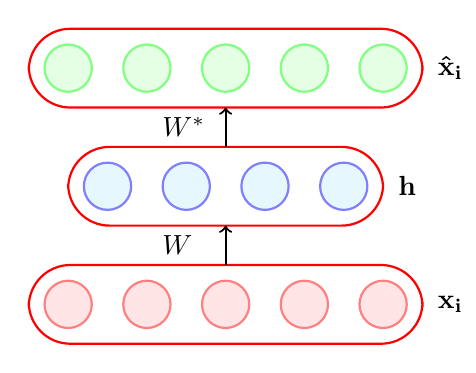
\begin{tikzpicture}

\node [input_neuron] (neuron01) at (6.5,4.5) {};
\node [input_neuron] (neuron02) at (7.5,4.5){};
\node [input_neuron] (neuron03) at (8.5,4.5) {};
\node [input_neuron] (neuron04) at (9.5,4.5) {};
\node [input_neuron] (neuron05) at (10.5,4.5) {};
\node [hidden_neuron] (neuron51) at (7,6) {} ;
\node [hidden_neuron] (neuron52) at (8,6)  {};
\node [hidden_neuron] (neuron53) at (9,6)  {};
\node [hidden_neuron] (neuron54) at (10,6)  {};

\node [output_neuron] (neuron11) at (6.5,7.5)  {};
\node [output_neuron] (neuron12) at (7.5,7.5)  {};
\node [output_neuron] (neuron13) at (8.5,7.5)  {};
\node [output_neuron] (neuron14) at (9.5,7.5)  {};
\node [output_neuron] (neuron15) at (10.5,7.5)  {};

\node[text width=0.01cm] at (11.2,4.5) {$\mathbf{x_i}$};
\node[text width=0.007cm] at (7.7,5.25) {$W$};
\node[text width=0.01cm] at (10.7,6) {$\mathbf{h}$};
\node[text width=0.007cm] at (7.7,6.75) {$W^*$};
\node[text width=0.01cm] at (11.2,7.5) {$\mathbf{\hat{x}_i}$};

\draw[red!100,thick,solid,rounded corners=15pt] (6,4) rectangle (11,5);
\draw[red!100,thick,solid,rounded corners=15pt] (6.5,5.5) rectangle (10.5,6.5);
\draw[red!100,thick,solid,rounded corners=15pt] (6,7) rectangle (11,8);



\draw[thick,->] (8.5,5) -- (8.5,5.5);

\draw[thick,->] (8.5,6.5) -- (8.5,7);



\end{tikzpicture}
\end{center}

            \vspace{-20pt}
            \begin{align*}
                \mathbf{h} &= g(W\mathbf{x_i} +\mathbf{b})\\
                \mathbf{\hat{x}_i} &= f(W^*\mathbf{h} +\mathbf{c})      
            \end{align*}


        \end{overlayarea}
    
        \column{0.5\textwidth}
        \begin{overlayarea}{\textwidth}{\textheight}
            \begin{itemize}\justifying
            		\item<2-> Consider the case when the inputs are real valued
                \item<3-> The objective of the autoencoder is to reconstruct $\mathbf{\hat{x}_i}$ to be as close to $\mathbf{x_i}$ as possible
                \item<4-> This can be formalized using the following objective function:
                \begin{align*}
                    & \min \limits_{W,W^*,\mathbf{c},\mathbf{b}}\hspace{0.5mm} \frac{1}{m}\sum_{i=1}^{m}\sum_{j=1}^{n} (\hat{x}_{ij}- x_{ij})^2 \\
                   \onslide<5-> {i.e., &  \min \limits_{W,W^*,\mathbf{c},\mathbf{b}}\hspace{0.5mm} \frac{1}{m}\sum_{i=1}^{m} (\mathbf{\hat{x}_{i}}- \mathbf{{x}_{i}})^T(\mathbf{\hat{x}_{i}}- \mathbf{x_{i}})}
                \end{align*}
                \item<6-> We can then train the autoencoder just like a regular feedforward network using backpropagation
                \item<7-> All we need is a formula for $\frac{\partial \mathscr{L(\theta)}}{\partial W^*}$ and $\frac{\partial \mathscr{L(\theta)}}{\partial W}$ which we will see now
            \end{itemize}
        \end{overlayarea}
    \end{columns}}
\end{frame}


\begin{frame}
	\small{
    \begin{columns}
        \column{0.4\textwidth}
        \begin{overlayarea}{\textwidth}{\textheight}
            \vspace{3pt}
            \tikzstyle{input_neuron}=[circle,draw=red!50,fill=red!10,thick,minimum size=6mm]
\tikzstyle{hidden_neuron}=[circle,draw=blue!50,fill=cyan!10,thick,minimum size=6mm]
\tikzstyle{output_neuron}=[circle,draw=green!50,fill=green!10,thick,minimum size=6mm]

\tikzstyle{input}=[circle,draw=black!50,fill=black!20,thick,minimum size=6mm]

\begin{center}
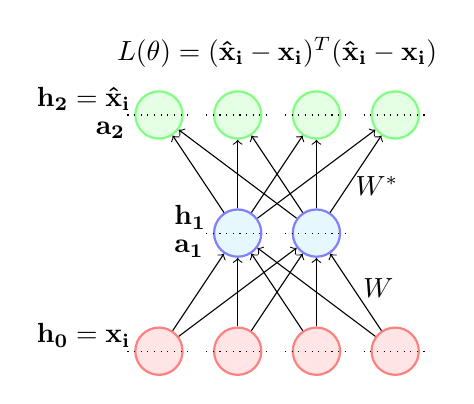
\begin{tikzpicture}


\node [input_neuron] (neuron01) at (6.5,4.5) {};
\node [input_neuron] (neuron02) at (7.5,4.5){};
\node [input_neuron] (neuron03) at (8.5,4.5) {};
\node [input_neuron] (neuron04) at (9.5,4.5) {};

\node [hidden_neuron] (neuron51) at (7.5,6) {} ;
\node [hidden_neuron] (neuron52) at (8.5,6)  {};

\node [output_neuron] (neuron11) at (6.5,7.5)  {};
\node [output_neuron] (neuron12) at (7.5,7.5)  {};
\node [output_neuron] (neuron13) at (8.5,7.5)  {};
\node [output_neuron] (neuron14) at (9.5,7.5)  {};

\node[] (lossexp) at (8,8.3)  {$\mathscr{L(\theta)} = (\mathbf{\hat{x}_{i}}- \mathbf{x_{i}})^T(\mathbf{\hat{x}_{i}}- \mathbf{x_{i}})$};

\node[text width=1.5cm] at (5.7,4.7) {$\mathbf{h_0}=\mathbf{x_i}$};
\node[text width=0.005cm] at (6.7,6.2) {$\mathbf{h_1}$};
\node[text width=0.005cm] at (6.7,5.8) {$\mathbf{a_1}$};
\node[text width=1.5cm] at (5.7,7.7) {$\mathbf{h_2}=\mathbf{\hat{x}_i}$};
\node[text width=0.005cm] at (5.7,7.3) {$\mathbf{a_2}$};
\node[text width=0.005cm] at (9.1,5.3) {$W$};
\node[text width=0.005cm] at (9,6.6) {$W^*$};

\draw [dotted] (6.1,4.5) -- (6.9,4.5);
\draw [dotted] (7.1,4.5) -- (7.9,4.5);
\draw [dotted] (8.1,4.5) -- (8.9,4.5);
\draw [dotted] (9.1,4.5) -- (9.9,4.5);

\draw [dotted] (7.1,6) -- (7.9,6);
\draw [dotted] (8.1,6) -- (8.9,6);

\draw [dotted] (6.1,7.5) -- (6.9,7.5);
\draw [dotted] (7.1,7.5) -- (7.9,7.5);
\draw [dotted] (8.1,7.5) -- (8.9,7.5);
\draw [dotted] (9.1,7.5) -- (9.9,7.5);
\draw[->](neuron01) -- (neuron51);
\draw[->](neuron01) -- (neuron52);
\draw[->](neuron02) -- (neuron51);
\draw[->](neuron02) -- (neuron52);
\draw[->](neuron03) -- (neuron51);
\draw[->](neuron03) -- (neuron52);
\draw[->](neuron04) -- (neuron51);
\draw[->](neuron04) -- (neuron52);

\draw[->](neuron51) -- (neuron11);
\draw[->](neuron51) -- (neuron12);
\draw[->](neuron51) -- (neuron13);
\draw[->](neuron51) -- (neuron14);

\draw[->](neuron52) -- (neuron11);
\draw[->](neuron52) -- (neuron12);
\draw[->](neuron52) -- (neuron13);
\draw[->](neuron52) -- (neuron14);

\end{tikzpicture}
\end{center}
            \begin{itemize}
            \item<2-> Note that the loss function is shown for only one training example.
            \end{itemize}
        \end{overlayarea}

        \column{0.6\textwidth}
        \begin{overlayarea}{\textwidth}{\textheight}
            \begin{itemize}\justifying %       $\displaystyle\begin{aligned}...\end{aligned}$
                \item<3-> $\displaystyle
                    \begin{aligned} 
                        \frac{\partial \mathscr{L(\theta)}}{\partial W^*} = 
                        \frac{\partial \mathscr{L(\theta)}}{\partial \mathbf{h_2}}
                        \boxed{\frac{\partial \mathbf{h_2}}{\partial \mathbf{a_2}}\frac{\partial \mathbf{a_2}}{\partial W^*}} 
                    \end{aligned}$ %\]
            \item<4-> $\displaystyle
                    \begin{aligned} 
                        \frac{\partial \mathscr{L(\theta)}}{\partial W} = 
                        \frac{\partial \mathscr{L(\theta)}}{\partial \mathbf{h_2}} 
                        \boxed{\frac{\partial \mathbf{h_2}}{\partial \mathbf{a_2}}\frac{\partial \mathbf{a_2}}{\partial \mathbf{h_1}}\frac{\partial \mathbf{h_1}}{\partial \mathbf{a_1}}\frac{\partial \mathbf{a_1}}{\partial W}} 
                    \end{aligned}$
            \item<5-> We have already seen how to calculate the expression in the boxes when we learnt backpropagation
                    \begin{align*}
                        \onslide<6->{\frac{\partial \mathscr{L(\theta)}}{\partial \mathbf{h_2}} &= \frac{\partial \mathscr{L(\theta)}}{\partial \mathbf{\hat{x}_i}}}\\
                        \onslide<7->{&=\nabla_{\mathbf{\hat{x}_i}}\{ (\mathbf{\hat{x}_{i}}- \mathbf{x_{i}})^T(\mathbf{\hat{x}_{i}}- \mathbf{x_{i}})\}}\\
                        \onslide<8->{&=2 (\mathbf{\hat{x}_i}-\mathbf{x_i})}
                    \end{align*}
            \end{itemize}
        \end{overlayarea}
    \end{columns}
    }
\end{frame}


\begin{frame}
    \small{
    \begin{columns}
        \column{0.46\textwidth}
        \begin{overlayarea}{\textwidth}{\textheight}
            \vspace{3pt}
       % \vspace{-0.75cm}
            \tikzstyle{input_neuron}=[circle,draw=red!50,fill=red!10,thick,minimum size=6mm]
\tikzstyle{hidden_neuron}=[circle,draw=blue!50,fill=cyan!10,thick,minimum size=6mm]
\tikzstyle{output_neuron}=[circle,draw=green!50,fill=green!10,thick,minimum size=6mm]

\tikzstyle{input}=[circle,draw=black!50,fill=black!20,thick,minimum size=6mm]

\begin{center}
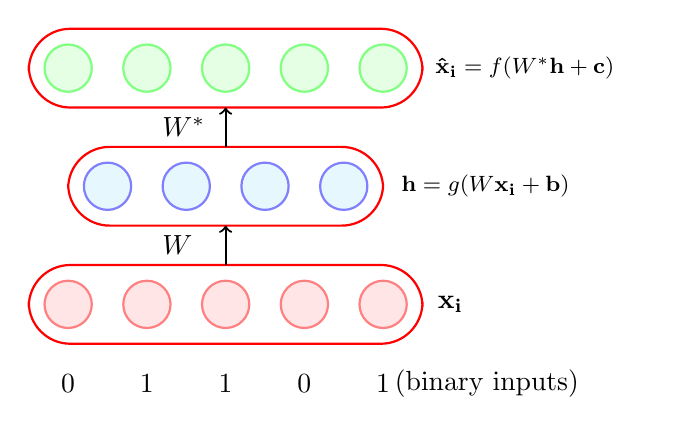
\begin{tikzpicture}

\node (input0) at (6.5,3.5) {0};
\node (input1) at (7.5,3.5) {1};
\node (input2) at (8.5,3.5){1};
\node (input3) at (9.5,3.5){0};
\node (input4) at (10.5,3.5){1};
\node [input_neuron] (neuron01) at (6.5,4.5) {};
\node [input_neuron] (neuron02) at (7.5,4.5){};
\node [input_neuron] (neuron03) at (8.5,4.5) {};
\node [input_neuron] (neuron04) at (9.5,4.5) {};
\node [input_neuron] (neuron05) at (10.5,4.5) {};
\node [hidden_neuron] (neuron51) at (7,6) {} ;
\node [hidden_neuron] (neuron52) at (8,6)  {};
\node [hidden_neuron] (neuron53) at (9,6)  {};
\node [hidden_neuron] (neuron54) at (10,6)  {};

\node [output_neuron] (neuron11) at (6.5,7.5)  {};
\node [output_neuron] (neuron12) at (7.5,7.5)  {};
\node [output_neuron] (neuron13) at (8.5,7.5)  {};
\node [output_neuron] (neuron14) at (9.5,7.5)  {};
\node [output_neuron] (neuron15) at (10.5,7.5)  {};

\node[text width=0.01cm] at (11.2,4.5) {$\mathbf{x_i}$};
\node[] at (11.8,6) {\footnotesize{$\mathbf{h}=g(W\mathbf{x_i}+\mathbf{b})$}};
\node[text width=0.007cm] at (7.7,5.25) {$W$};
%\node[] at (11.2,8.5) {$\hat{x} = f(W \times h(x) + c)$};
\node[text width=0.007cm] at (7.7,6.75) {$W^*$};
\node[] at (12.3,7.5) {\footnotesize{$\mathbf{\hat{x}_i}=f(W^*\mathbf{h}+\mathbf{c})$}};
\node[text width=3.1cm] at (12.2,3.5) {(binary inputs)};

\draw[red!100,thick,solid,rounded corners=15pt] (6,4) rectangle (11,5);
\draw[red!100,thick,solid,rounded corners=15pt] (6.5,5.5) rectangle (10.5,6.5);
\draw[red!100,thick,solid,rounded corners=15pt] (6,7) rectangle (11,8);

\draw[thick,->] (8.5,5) -- (8.5,5.5);

\draw[thick,->] (8.5,6.5) -- (8.5,7);


\end{tikzpicture}
\end{center}

            \vspace{-0.4cm}

            \only<5->
            {
                What value of $\hat{x}_{ij}$ will minimize this function?
            }
            \vspace{-5pt}
            \begin{itemize}
                \item<6-> If $x_{ij} = 1$ ?
                \item<7-> If $x_{ij} = 0$ ?
            \end{itemize}
            \only<9->
            {
                Indeed the above function will be minimized when $\hat{x}_{ij}=x_{ij}$ ! %(which is exactly what we desire)
            }
        \end{overlayarea}

        \column{0.52\textwidth}
        \begin{overlayarea}{\textwidth}{\textheight}
        \vspace{0.2pt}
            \begin{itemize} 

                \item<2-> Consider the case when the inputs are binary
                \item <3-> We use a sigmoid decoder which will produce outputs between 0 and 1, and can be interpreted as probabilities.
                \item <4->For a single n-dimensional $i^{th}$ input we can use the following loss function
                \vspace{-0.1in}
                \begin{align*}
                \min \{ -\sum\limits_{j=1}^n(x_{ij}\log\hat{x}_{ij} + (1-x_{ij}) \log(1- \hat{x}_{ij})) \}
                \end{align*}
                \vspace{-0.2in}
                %\item <5-> The above function is simply the sum of cross entropy of $k$ Bernoulli distributions
                \item<8-> Again we need is a formula for $\frac{\partial \mathscr{L(\theta)}}{\partial W^*}$ and $\frac{\partial \mathscr{L(\theta)}}{\partial W}$ to use backpropagation 
            \end{itemize}
        \end{overlayarea}
    \end{columns}
    }
\end{frame}

\begin{frame}
    \begin{columns}
        \column{0.5\textwidth}
        \begin{overlayarea}{\textwidth}{\textheight}
            \vspace{2pt}
            \tikzstyle{input_neuron}=[circle,draw=red!50,fill=red!10,thick,minimum size=6mm]
\tikzstyle{hidden_neuron}=[circle,draw=blue!50,fill=cyan!10,thick,minimum size=6mm]
\tikzstyle{output_neuron}=[circle,draw=green!50,fill=green!10,thick,minimum size=6mm]

\tikzstyle{input}=[circle,draw=black!50,fill=black!20,thick,minimum size=6mm]

\begin{center}
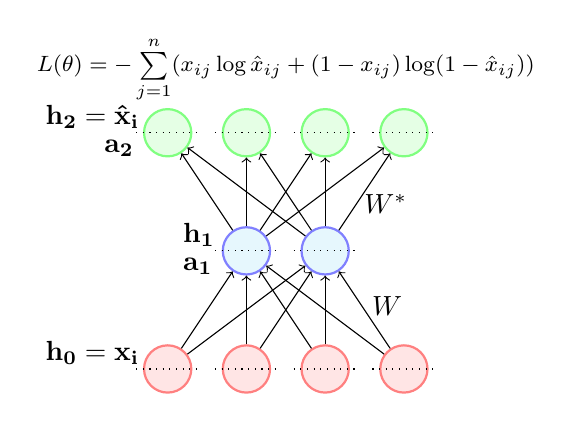
\begin{tikzpicture}


\node [input_neuron] (neuron01) at (6.5,4.5) {};
\node [input_neuron] (neuron02) at (7.5,4.5){};
\node [input_neuron] (neuron03) at (8.5,4.5) {};
\node [input_neuron] (neuron04) at (9.5,4.5) {};

\node [hidden_neuron] (neuron51) at (7.5,6) {} ;
\node [hidden_neuron] (neuron52) at (8.5,6)  {};

\node [output_neuron] (neuron11) at (6.5,7.5)  {};
\node [output_neuron] (neuron12) at (7.5,7.5)  {};
\node [output_neuron] (neuron13) at (8.5,7.5)  {};
\node [output_neuron] (neuron14) at (9.5,7.5)  {};

\node[] (lossexp) at (8,8.3)  {\footnotesize{$ \mathscr{L(\theta)} =  -\sum\limits_{j=1}^n(x_{ij}\log\hat{x}_{ij} + (1-x_{ij}) \log(1-\hat{x}_{ij})) $}};

\node[text width=1.5cm] at (5.7,4.7) {$\mathbf{h_0}=\mathbf{x_i}$};
\node[text width=0.005cm] at (6.7,6.2) {$\mathbf{h_1}$};
\node[text width=0.005cm] at (6.7,5.8) {$\mathbf{a_1}$};
\node[text width=1.5cm] at (5.7,7.7) {$\mathbf{h_2}=\mathbf{\hat{x}_i}$};
\node[text width=0.005cm] at (5.7,7.3) {$\mathbf{a_2}$};
\node[text width=0.005cm] at (9.1,5.3) {$W$};
\node[text width=0.005cm] at (9,6.6) {$W^*$};

\draw [dotted] (6.1,4.5) -- (6.9,4.5);
\draw [dotted] (7.1,4.5) -- (7.9,4.5);
\draw [dotted] (8.1,4.5) -- (8.9,4.5);
\draw [dotted] (9.1,4.5) -- (9.9,4.5);

\draw [dotted] (7.1,6) -- (7.9,6);
\draw [dotted] (8.1,6) -- (8.9,6);

\draw [dotted] (6.1,7.5) -- (6.9,7.5);
\draw [dotted] (7.1,7.5) -- (7.9,7.5);
\draw [dotted] (8.1,7.5) -- (8.9,7.5);
\draw [dotted] (9.1,7.5) -- (9.9,7.5);
\draw[->](neuron01) -- (neuron51);
\draw[->](neuron01) -- (neuron52);
\draw[->](neuron02) -- (neuron51);
\draw[->](neuron02) -- (neuron52);
\draw[->](neuron03) -- (neuron51);
\draw[->](neuron03) -- (neuron52);
\draw[->](neuron04) -- (neuron51);
\draw[->](neuron04) -- (neuron52);

\draw[->](neuron51) -- (neuron11);
\draw[->](neuron51) -- (neuron12);
\draw[->](neuron51) -- (neuron13);
\draw[->](neuron51) -- (neuron14);

\draw[->](neuron52) -- (neuron11);
\draw[->](neuron52) -- (neuron12);
\draw[->](neuron52) -- (neuron13);
\draw[->](neuron52) -- (neuron14);

\end{tikzpicture}
\end{center}

            \vspace{-0.35cm}
			
		\begin{equation*} 
\setstackgap{L}{20pt}
 \onslide<6->{\frac{\partial \mathscr{L(\theta)}}{\partial \mathbf{h_2}} = \parenMatrixstack{
\frac{\partial \mathscr{L(\theta)}}{\partial h_{21}}  \cr
\frac{\partial \mathscr{L(\theta)}}{\partial h_{22}} \cr
\vdots \cr
\frac{\partial \mathscr{L(\theta)}}{\partial h_{2n}}
}}
\end{equation*}

        \end{overlayarea}

        \column{0.5\textwidth}
        \begin{overlayarea}{\textwidth}{\textheight}
            \begin{itemize}
                \item<2-> $\displaystyle
                        \begin{aligned}
                            \frac{\partial \mathscr{L(\theta)}}{\partial W^*} = 
                            \frac{\partial \mathscr{L(\theta)}}{\partial \mathbf{h_2}}\frac{\partial \mathbf{h_2}}{\partial \mathbf{a_2}}\boxed{\frac{\partial \mathbf{a_2}}{\partial W^*}}
                        \end{aligned}$
                \item<3-> $\displaystyle
                        \begin{aligned}
                            \frac{\partial \mathscr{L(\theta)}}{\partial W} = 
                            \frac{\partial \mathscr{L(\theta)}}{\partial \mathbf{h_2}}\frac{\partial \mathbf{h_2}}{\partial \mathbf{a_2}}\boxed{\frac{\partial \mathbf{a_2}}{\partial \mathbf{h_1}}\frac{\partial \mathbf{h_1}}{\partial \mathbf{a_1}}\frac{\partial \mathbf{a_1}}{\partial W}}
                        \end{aligned}$
                \item<4-> We have already seen how to calculate the expressions in the square boxes when we learnt BP
                \item<5->The first two terms on RHS can be computed as:
                		$\displaystyle                        
                        \begin{aligned}
                            \frac{\partial \mathscr{L(\theta)}}{\partial h_{2j}} &= -\frac{x_{ij}}{\hat{x}_{ij}} + \frac{1 - x_{ij}}{1 - \hat{x}_{ij}}\\
                            \frac{\partial h_{2j}}{\partial a_{2j}} &= \sigma(a_{2j}) (1 - \sigma(a_{2j})) %<$workout the expression$>
                        \end{aligned}$
            \end{itemize}
        \end{overlayarea}
    \end{columns}
\end{frame}